\chapter{Validation croisée des simulations}

\section{Convertisseur CC-CC 4 quadrants formé de 2 convertisseurs 3 niveaux NPC}

Le premier sous-système est celui du convertisseur CC-CC 4 quadrants formé de 2 convertisseurs triphasés 3 niveaux NPC avec une commande par MLI à 333Hz, intercalée de 120$^\circ$ par phase. La fréquence vue à la charge est la même que la fréquence de commande de l'AFE, soit 1kHz. L'entrelacement  des commandes permet de réduire les valeurs RMS et moyennes des courants dans les différents bras des convertisseurs. La tension maximale vue des interrupteurs est abaissée à la moitié de la tension du bus CC, ce qui présente un net avantage de dimensionnement. Le sous-système du DCP/DCN permet de remplir l'exigence d'alimenter les électroaimants avec une forme de courant précise. De plus, la puissance moyenne et maximale doivent être similaires à celles prévues par le CERN (18MW crête et 5.4MW moyenne). Les simulations ont été implantées sous SPS et PSIM, le simulateur d'OPAL-RT n'étant pas disponible à temps. Les résultats comparatifs du courant dans la charge sont présentés à la figure \ref{DC_ch_cou_1}. On remarque premièrement que les 2 simulateurs permettent de suivre la consigne de courant demandée. Par la suite, lorsqu'on observe le courant en maintient à 6kA, on remarque qu'il y a une légère différence de fréquence entre les 2 signaux, de l'ordre d'environ 110Hz. La différence est apportée par l'implémentation des filtres dans les 2 simulateurs ainsi que par les algorithmes utilisés afin de solutionner les matrices d'équation d'états (SPS) et les matrices d'admittances nodales (PSIM). De plus, les algorithmes de détection des passages par 0 ne sont pas exactement similaires. SPS utilise une discrétisation par la méthode de Tustin et PSIM une méthode trapézoïdale pure. Ce faisant, vu la quantité de composantes et le nombre de commutations élevées (36 interrupteurs commandés), il est normal d'observer des différences ponctuelles. On constante cependant que les amplitudes observées sont identiques et que les signaux reviennent en phase périodiquement. Les formes d'ondes de courant en montée initiale et en montée rapide permettent de constater que la réponse globale des simulateurs est similaire et qu'ils présentent un comportement analogue.

\paragraph{} La figure \ref{DC_IG_ten_1} présente la tension aux bornes d'un IGBT du DCP/DCN dans les 2 simulateurs. On remarque que les patrons de tensions et les durées de conduction sont les identiques, de même que les amplitudes, mais qu'il y a un décalage de l'une des simulations par rapport à l'autre, ce qui explique les différences ponctuelles. 

\paragraph{}Pour ce qui est du sous-système formé par le DCP/DCN, on comprend que la commande des interrupteurs représente le fonctionnement désiré, qu'elle permet de remplir l'exigence d'alimenter les électroaimants de l'accélérateur de particules avec une forme de courant précise et une fréquence de modulation équivalente de 1kHz. Aussi, la correspondance du fonctionnement dans PSIM et dans SPS a été vérifiée par des comparaisons à l'échelle de la modulation. 

\begin{figure}[htb]
\centering
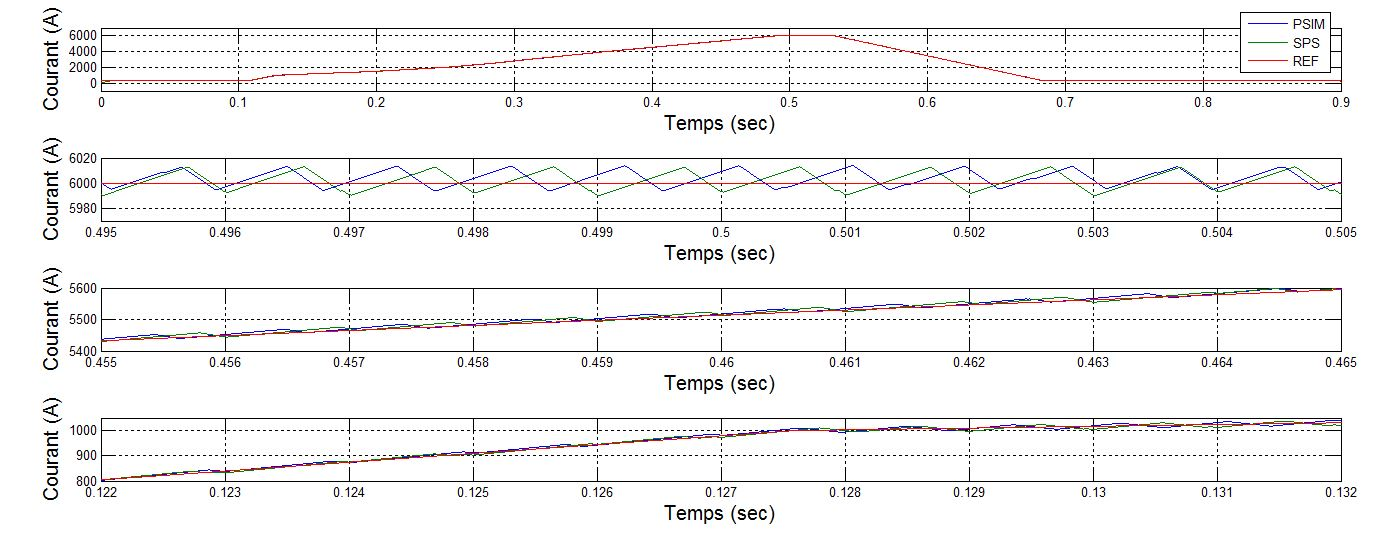
\includegraphics[scale=0.5]{fig/DCPDCN/DCPCourantCharge1u.jpg}
\caption{Courant traversant la charge sur PSIM et SPS pour un pas de calcul de 1$\mu$s pour le DCP/DCN}
\label{DC_ch_cou_1}
\end{figure}

\begin{figure}[htb]
\centering
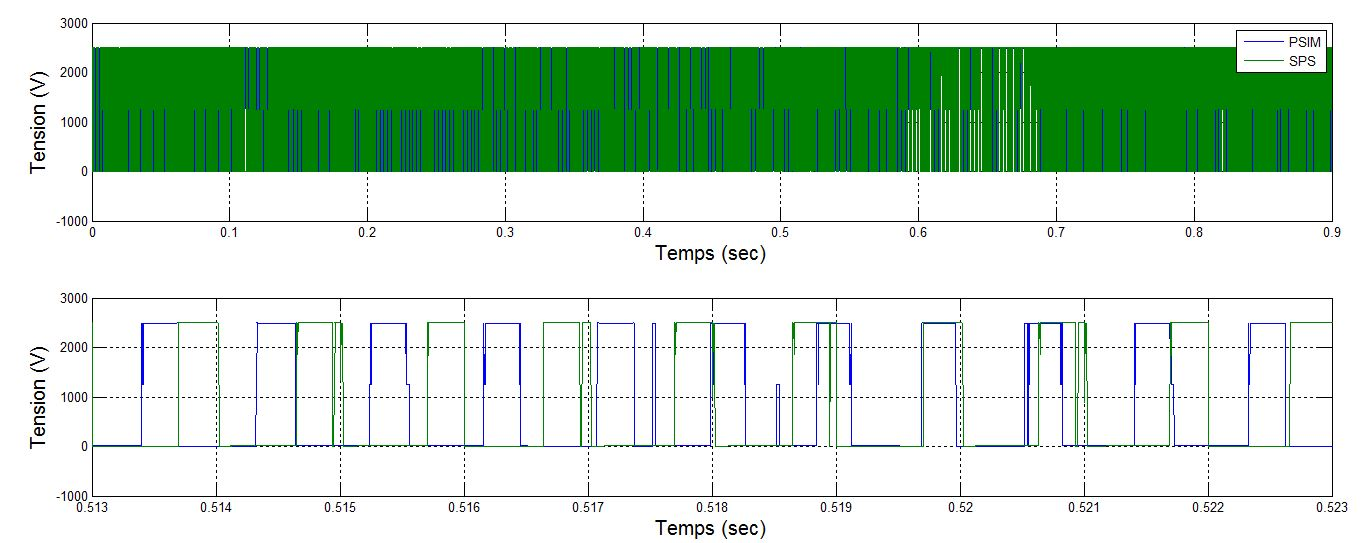
\includegraphics[scale=0.5]{fig/DCPDCN/DCPTensionIGBT1u.jpg}
\caption{Tension aux bornes d'un IGBT sur PSIM et SPS pour un pas de calcul de 1$\mu$s pour le DCP/DCN}
\label{DC_IG_ten_1}
\end{figure}

\section{AFE 3 niveaux NPC avec contrôle par MLI}
Le second sous-système est celui de l'AFE 3 niveaux NPC triphasé avec contrôle par MLI débitant sur une charge RC équivalente. Ce sous-système permet de remplir l'exigence de redresser le signal d'entrée du transformateur et de fournir une puissance moyenne maximale de 2.7MW et une puissance crête maximale de 3.6MW tout en maintenant la phase du courant nulle par rapport à la tension.
\begin{figure}[htb]
\centering
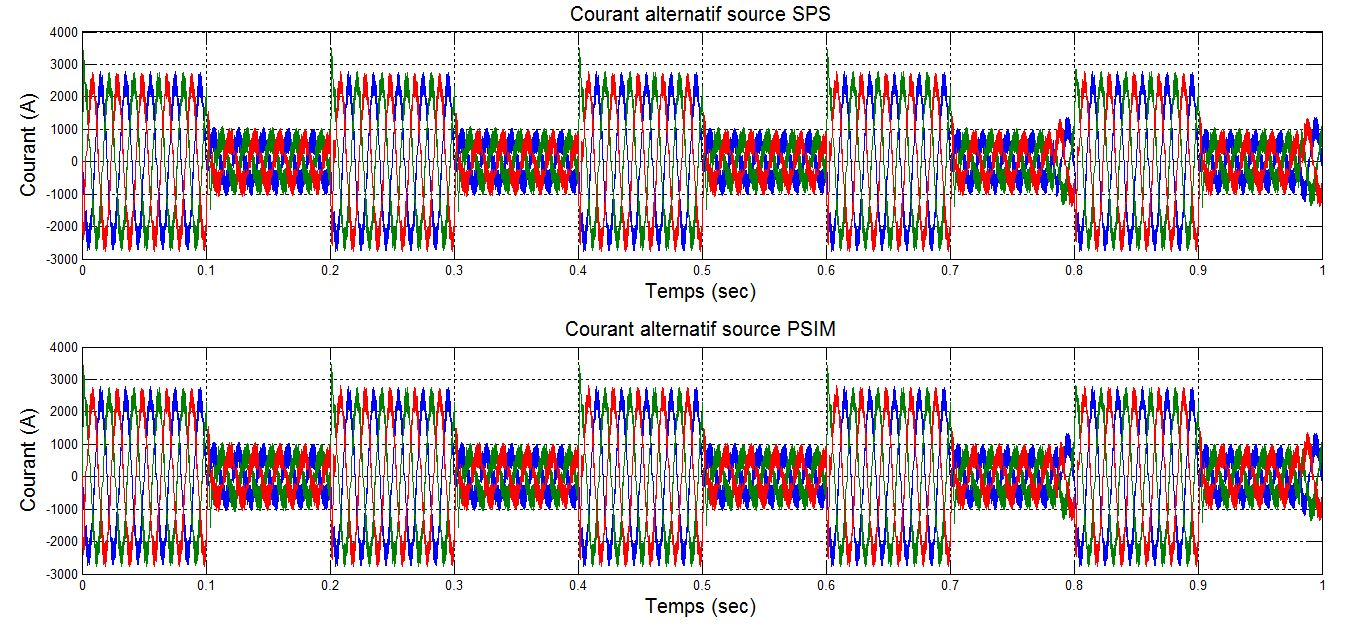
\includegraphics[scale=0.5]{fig/coual_afe.jpg}
\caption{Le courant d'entré à 1$\mu$s pour l'AFE sur charge RC}
\label{AF_RC_cou}
\end{figure}




\begin{figure}[htb]
\centering
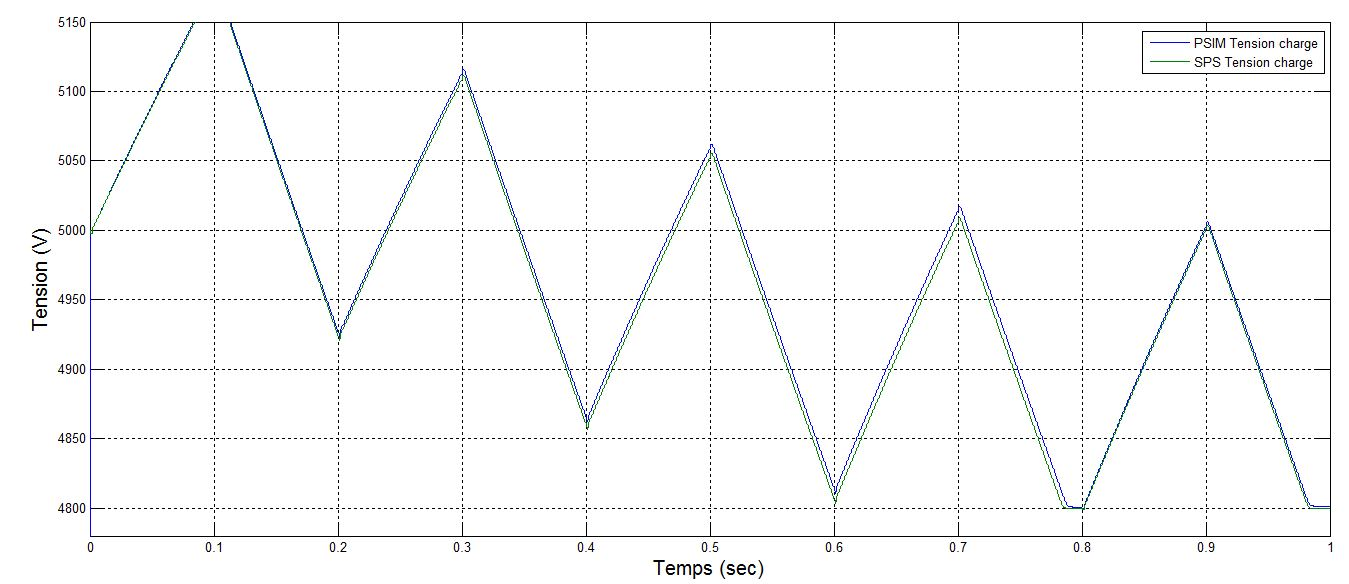
\includegraphics[scale=0.5]{fig/ten_afe.jpg}
\caption{La tension à la charge à 1$\mu$s pour l'AFE sur charge RC}
\label{AF_RC_ten}
\end{figure}



\begin{figure}[htb]
\centering
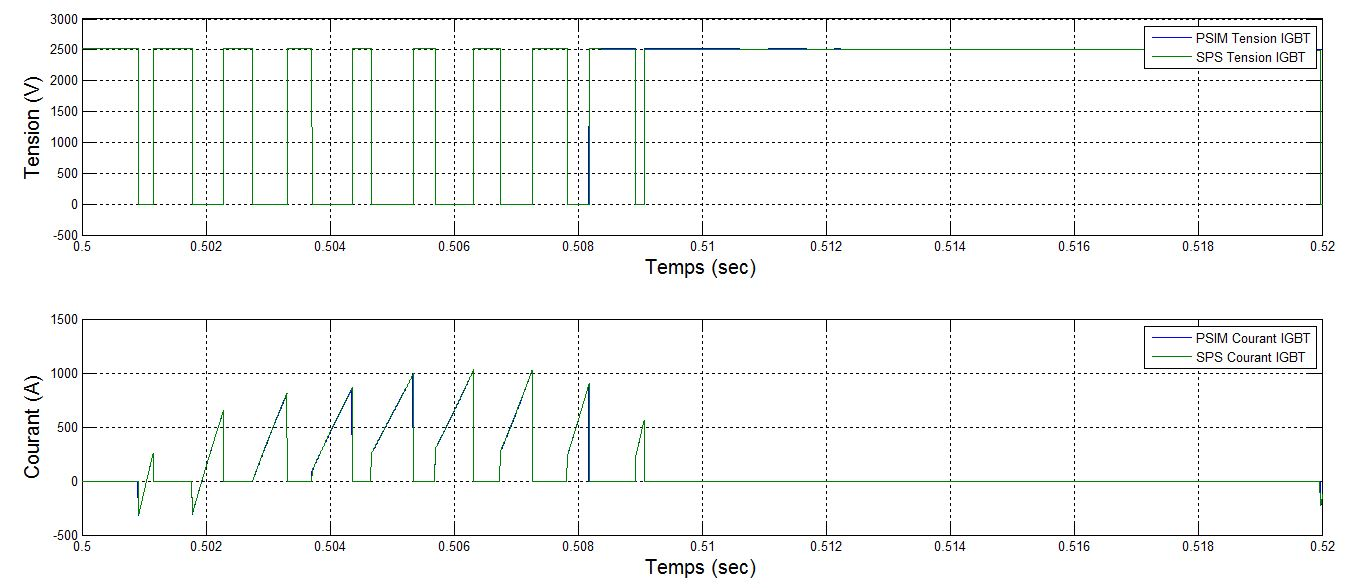
\includegraphics[scale=0.5]{fig/com_afe.jpg}
\caption{La tension et le courant au bornes d'un IGBT à 1$\mu$s pour l'AFE sur charge RC}
\label{AF_RC_igbt}
\end{figure}

\section{AFE 3 niveaux NPC avec contrôle par MLI avec convertisseur CC-CC formé de 2 cellules NPC 3 niveaux}

\begin{figure}[htb]
\centering
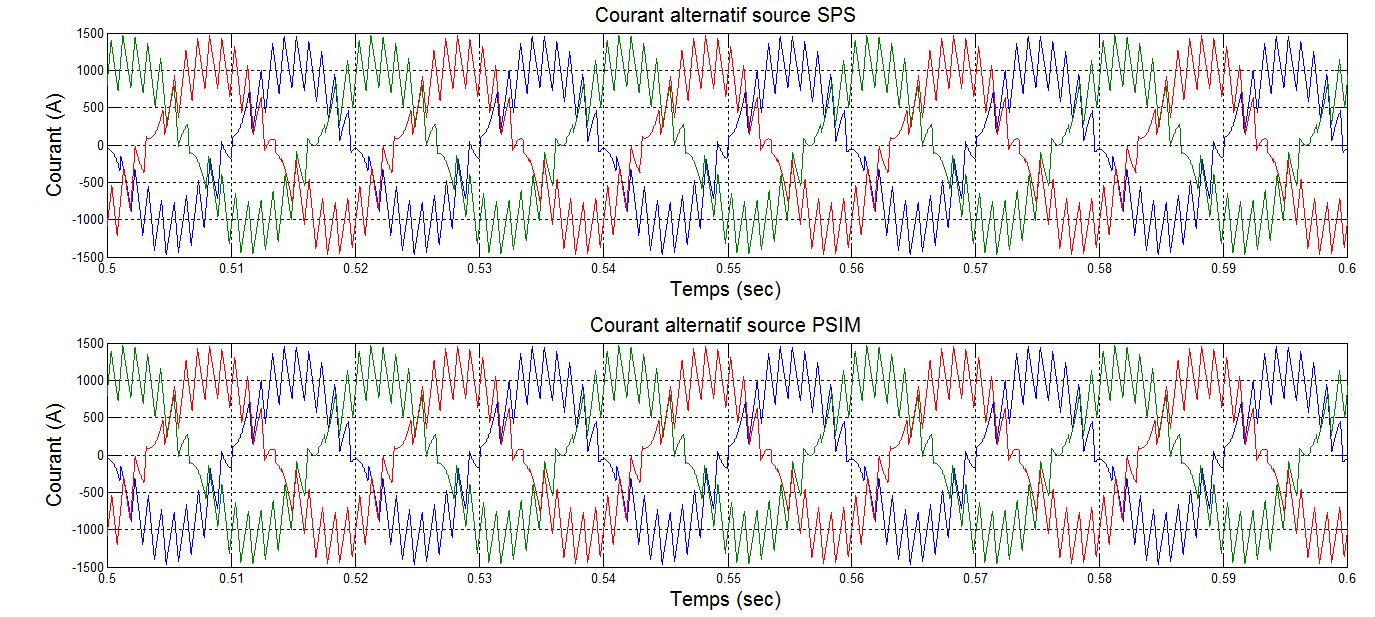
\includegraphics[scale=0.5]{fig/DCP_AFE/1u/cour_al.jpg}
\caption{Le courant d'entrée de l'AFE pour un pas de calcul de 1$\mu$s}
\label{AF_DC_cou1}
\end{figure}


\begin{figure}[htb]
\centering
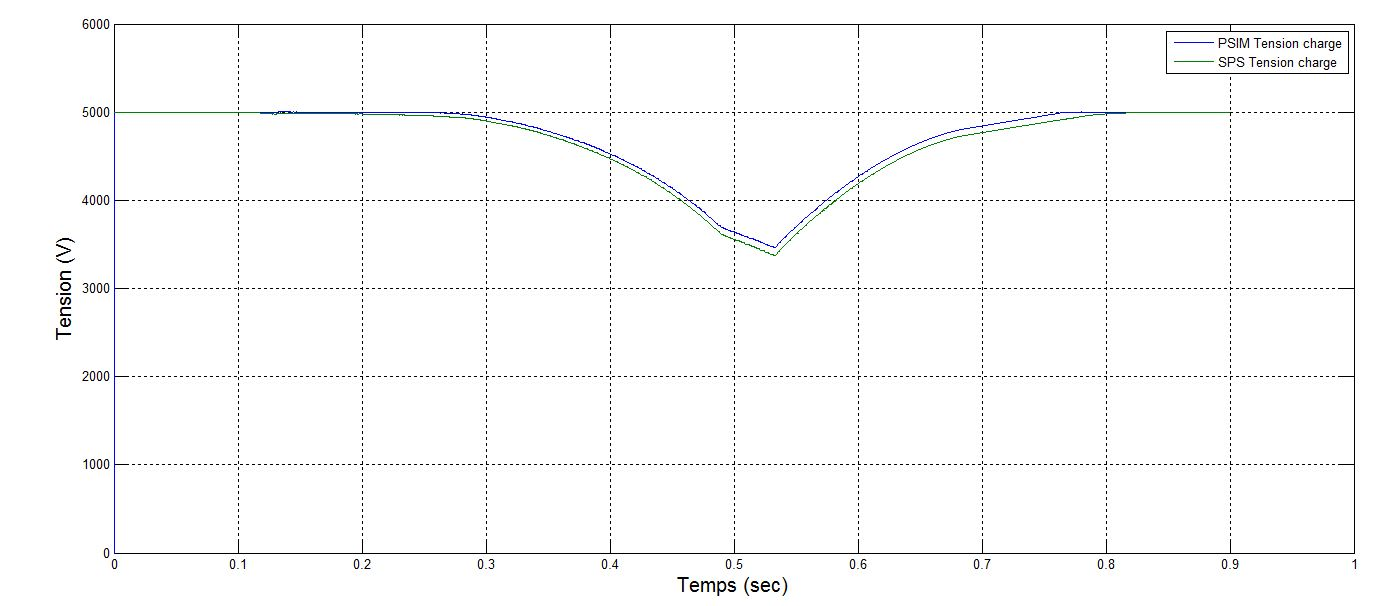
\includegraphics[scale=0.5]{fig/DCP_AFE/1u/ten_bus.jpg}
\caption{La tension du bus CC pour un pas de calcul de 1$\mu$s}
\label{AF_DC_vch1}
\end{figure}

\begin{figure}[htb]
\centering
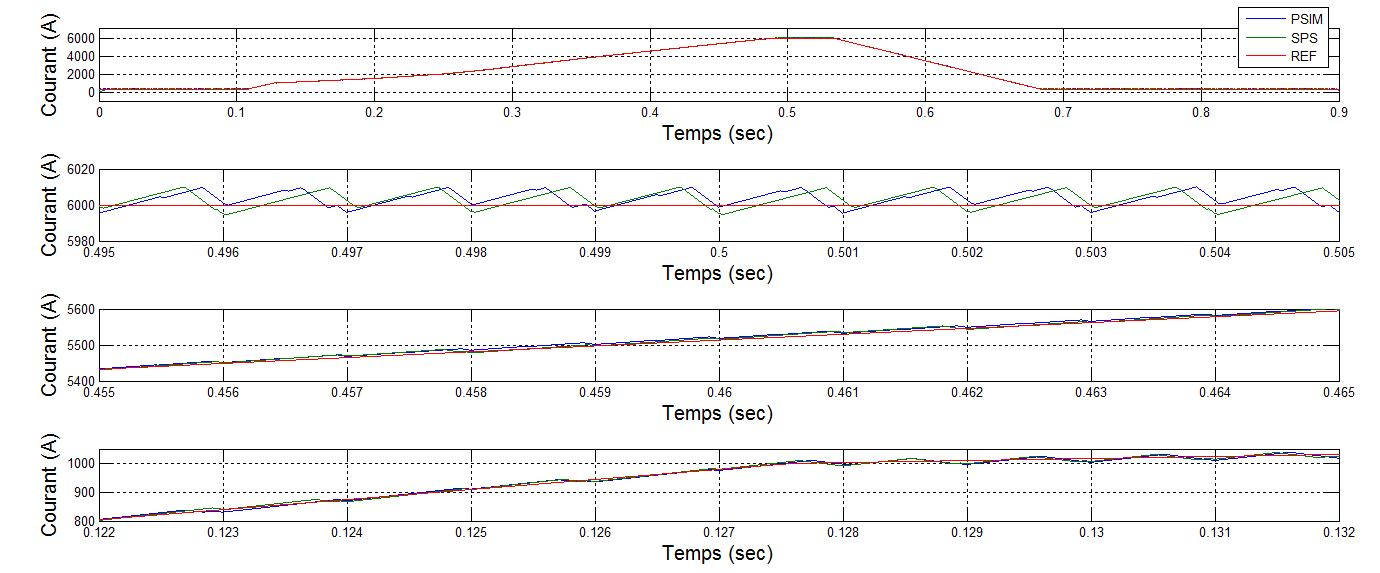
\includegraphics[scale=0.5]{fig/DCP_AFE/1u/cour_ch.jpg}
\caption{Le courant aux bornes des électroaimants pour un pas de calcul de 1$\mu$s}
\label{AF_DC_CHA1}
\end{figure}

\begin{figure}[htb]
\centering
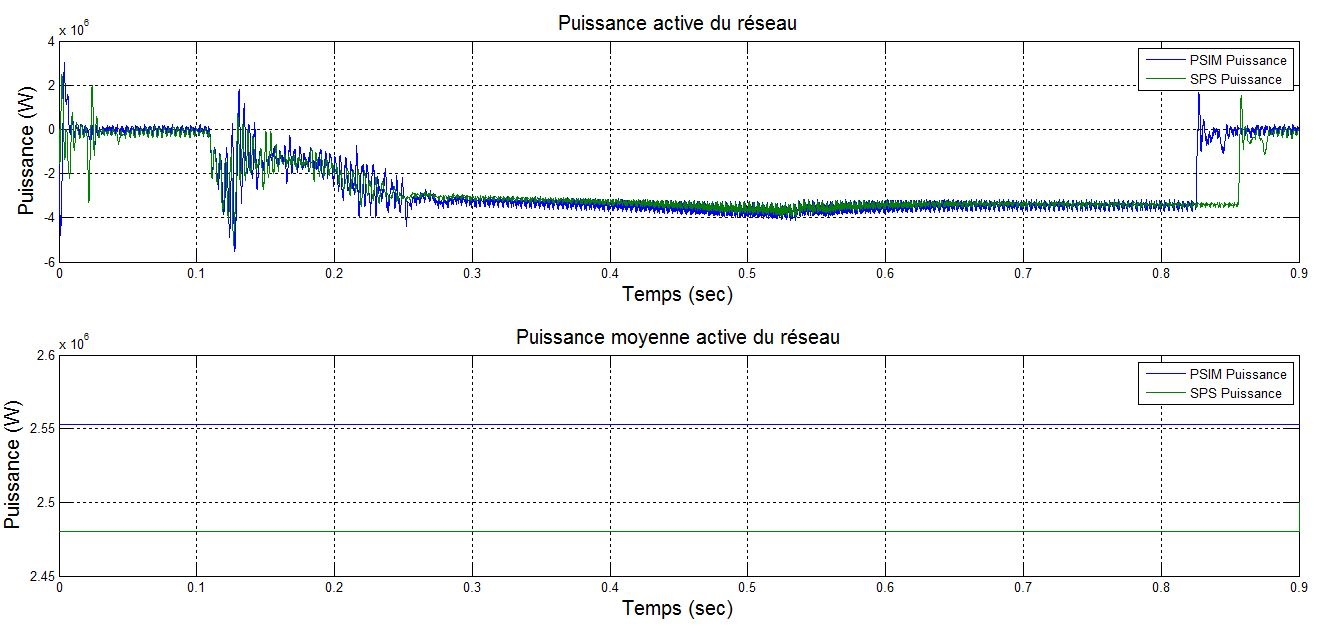
\includegraphics[scale=0.5]{fig/DCP_AFE/1u/PUI.jpg}
\caption{La puissance délivrée par le réseau alternatif pour un pas de calcul de 1$\mu$s}
\label{AF_DC_CHA1}
\end{figure}